%!TEX root = ../../../main.tex
%%---------------------------------------------------------------------------
\section{Robot motion and grasping}
\label{sec:rc_grasp}
%%---------------------------------------------------------------------------
When a brick is detected and is in agreement with the order it needs to be picked and moved from the conveyor belt to the tipper of the mobile robot. This requires a number of robot and gripper actions. 

Figure \ref{fig:rc_grasp} shows the steps taken when a brick is to be picked. 

	\begin{figure}[H]
		\centering
	    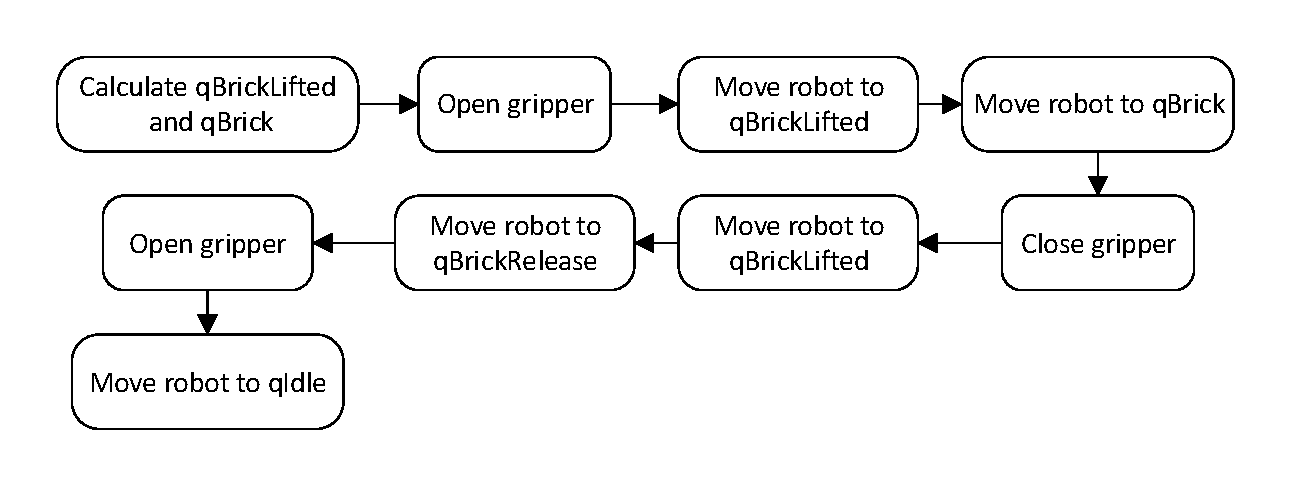
\includegraphics[width=0.95\textwidth]{rc_grasp_steps}
	    \caption{Steps performed when a Lego brick is to be picked}
		\label{fig:rc_grasp}
	\end{figure}
		
The idle position of the robot is with the z-axis of the camera frame aligned with the z-axis of the conveyor frame but with a certain distance displacement, as seen in figure \ref{fig:rc_frames}.

The calculation of \textit{qBrickLifted} and \textit{qBrick} includes inverse kinematics calculations used in order to get the position of the brick in the conveyor frame to a position in the robot frame with respect to the gripper. The configurations respectively represents the one in which the gripper and robot is aligned for grasping, but with a small offset in the z-axis and the configuration without the z-axis offset in which the gripper is in position for closing.  

No path planning is used in the process since the work-cell is static. The area in which bricks can be picked from is limited thus eliminating wrongly detected bricks resulting in collision. 

